\section{Hypertension} \label{sec:hypertension}

Et blodtryk afhænger af den kraft, som hjertet udøver, når blodet pumpes rundt i kroppen \citep{martini2015}. Ved hypertension bliver blodet pumpet igennem pulsårerne med et højere tryk end, hvad der er defineret som normalt. Yderligere afhænger dette tryk af den arterielle karmodstand, da der ved hypertension er et normalt hjerteminutvolumen \citep{olsen2015}. 
Blodtrykket er karakteriseret ved et systolisk og et diastolisk blodtryk, som henholdsvis er trykket i arterierne, når hjertet trækker sig sammen under systole, og trykket mellem to hjerteslag under diastole. Blodtryk skrives som 'systole/diastole' og måles i enheden millimeter kviksølv (mmHg). Det anbefales, at blodtrykket er under 140/90 mmHg, hvor et blodtryk over denne grænse betegnes hypertension. Et blodtryk mellem 120/80 og 139/89 mmHg kaldes et 'højt normalt blodtryk', og der bør gøres opmærksom på dette for at undgå hypertension \cite{martini2015}.
  
Ved måling af blodtryk under konsultationer af den danske befolkning i aldersgruppen 20 - 89 år ses, at 25,7 \% lider af hypertension, mens det ved hjemmeblodtryksmåling er 22,3 \% \cite{kronborg2008}. På \autoref{fig:ihyp_praevalens} illustreres  prævalensen af hypertension i Danmark fordelt på forskellige aldersgrupper og køn. Det fremgår af figuren, hvordan prævalensen stiger med alderen, og hvor stor en procentdel af den voksne danske befolkning, der er diagnosticeret med sygdommen.

\begin{figure}[H]
\centering
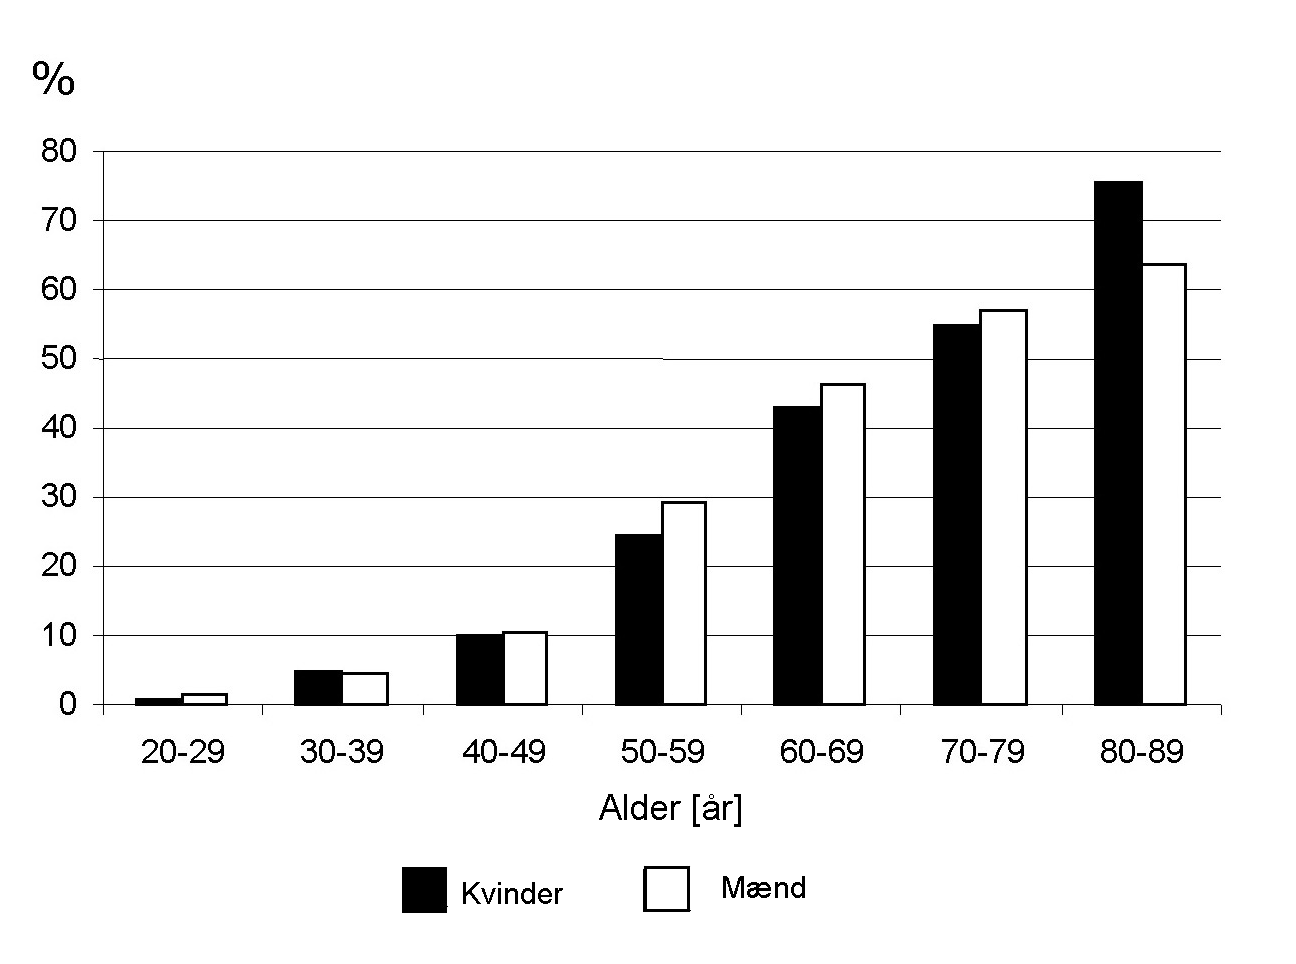
\includegraphics[width=0.7\textwidth]{figures/hyp_praevalens}
\caption{Prævalens af hypertension i Danmark fordelt på alder og køn \citep{kronborg2008}.}
\label{fig:ihyp_praevalens}
\end{figure}

\noindent
Omkring 30 \% er ikke bevidste om, at de lider af hypertension. Dette skyldes, at der ofte ikke er tydelige symptomer på lidelsen \cite{kronborg2008}. Symptomer, der kan forekomme ved hypertension, er træthed, hovedpine, næseblod, hjertebanken og åndenød ved anstrengelse. Idet hypertension i de fleste tilfælde ikke medfører symptomer, opdages lidelsen ofte ved et tilfælde \cite{olsen2015}.
Der er en række sundhedsmæssige risici forbundet med hypertension, idet sygdommen medfører et øget pres på kroppens blodkar, hvilket forøger risikoen for udvikling af arteriesklerose, aneurismer, hjerteanfald og hjerteinsufficiens samt apopleksi. Længerevarende hypertension er af denne grund ofte årsag til kronisk nyresvigt og hjertekarsygdomme \cite{martini2015}. Det kan være svært at estimere tal for dødeligheden som følge af hypertension, da patienterne ofte dør af følgevirkninger, og årsagen til dødsfald kan derfor være uklar. Ifølge Statens Institut for Folkesundhed er omkring 4 \% af alle dødsfald i Danmark relateret til hypertension \cite{juel2006}.
 
På trods af de sundhedsmæssige risici ved hypertension får 2/3 af de diagnosticerede patienter ikke tilstrækkelig behandling således, at de kan opnå det anbefalede blodtryk \cite{paulsen2012}.

% Martinibogen skal i kildelisten.

I de fleste tilfælde er årsagen til hypertension ukendt, men der er patientgrupper, der har særlig høj risiko for at udvikle hypertension. En anden lidelse, der ofte forbindes med hypertension, er diabetes. De to lidelser er begge resultatet af metabolisk syndrom, som er forstyrrelser i kroppens metabolisme og forekommer ofte grundet overvægt \cite{cheung2012}.

Behandling af hypertension kan ske farmakologisk eller non-farmakologisk. Ved farmakologisk behandling tages der højde for graden af hypertension, samt hvorvidt der er udviklet følgesygdomme. Alle patienter med hypertension bør, jævnfør anbefalinger fra \citeauthor{bech2015}, behandles non-farmakologisk, hvilket betyder, at de får en række anbefalinger fra lægen, der bør følges. Herunder blandt andet ændring af motions- og kostvaner. Hypertensive patienter bør jævnligt, ved konsultationer, få kontrolleret blodtrykket, hvor lægen eller sygeplejersken desuden kan følge op på patientens vægt, kost og aktivitetsniveau \cite{lodberg2016, bech2015}. 

\subsection{Påvirkende faktorer i relation til hypertension}

Fysisk aktivitet er generelt anset som værende relateret til blodtryk og hypertension, og er ligeledes en del af den primære behandling og kontrol af hypertension \citep{pescatello2004, fagard2006}.
Et studie baseret på 72 forsøg og 105 andre studier viste, at ved fysisk aktivitet falder hvileblodtryk med 3,0/2,4 mmHg og ambulant målt blodtryk med 3,3/3,5 mmHg. 
Hypertensive patienter fra 30 patientgrupper viste en yderligere reduktion i blodtryk på 6,9/4,9 mmHg end andre forsøgspersoner 1,9/1,6 mmHg \citep{fagard2006}. 
Dette er generelt blandt hypertensive patienter, at jo højere blodtryk patienten har, des større reduktion kan opnås ved fysisk aktivitet \citep{pedersen2011, pescatello2004}.

Den reducerende effekt af blodtrykket kan ses op til 22 timer efter en udholdenhedsøvelse, hvortil det anses, at der ved relativt få træningssessioner kan opnås en blodtryksreducerende effekt i døgnets 24 timer \citep{pescatello2004}.

%Der er forskellige faktorer relateret til reduktion i blodtryk. Flere faktorer fremgår i \autoref{sec:FoeglerAfFiA}, hvor fysisk aktivitet kan have modsatrettet virkning i forhold til effekterne ved fysisk inaktivitet. Dette ses for eksempel som en øget insulinfølsomhed i musklerne ved træning, hvor mængden af insulin i blodet falder. Dette kan påvirke hypertension, da det ofte optræder i sammenhæng med insulinresistens og hyperinsulinæmien \citep{pedersen2011}.

I \autoref{sec:FoeglerAfFiA} beskrives de fysiologiske følger til fysisk inaktivitet, hvortil fysisk aktivitet har en modsatrettet virkning på blandt andet hypertension \citep{pedersen2011}. Ved fysisk aktivitet øges kapillariseringen, hvorved den perifere modstand i kredsløbet mindskes og blodvolumenet øges. Yderligere forøges hjertets slagvolumen, hvorved hjertets arbejde reduceres. På denne måde kan fysisk aktivitet bruges i behandlingen af hypertension \citep{andersen2001}.

Normalt kan hypertension behandles i almen praksis, men i tilfælde af behandlingsresistent hypertension, hvor blandt andet motion, kostændringer, formindsket alkoholindtag og farmakologisk antihypertensiv behandling ikke kan udrede sygdommen, vil patienterne opleve at blive videresendt til en hypertensionsklinik \cite{lodberg2016, bech2015}.

Med intention om at spare sundhedsvæsenet penge og forbedre hypertensive patienters livskvalitet, ved blandt andet at skære ned på forbruget af medicin, samt mindske bivirkninger herfra, anses det af ovenstående grund for at være relevant at undersøge, hvorvidt videresendelsen af hypertensive patienter i almen praksis kan begrænses. Så vidt muligt bør begrænsningen ske gennem forbedringer i behandlingsmetoderne hos den praktiserende læge ved at skabe større mulighed for monitorering af hypertensionsrelaterede vaner. 